\documentclass[a4paper]{article} 
\addtolength{\hoffset}{-2.25cm}
\addtolength{\textwidth}{4.5cm}
\addtolength{\voffset}{-3.25cm}
\addtolength{\textheight}{5cm}
\setlength{\parskip}{0pt}
\setlength{\parindent}{0in}

%----------------------------------------------------------------------------------------
%	PACKAGES AND OTHER DOCUMENT CONFIGURATIONS
%----------------------------------------------------------------------------------------

\usepackage{blindtext} % Package to generate dummy text
\usepackage{charter} % Use the Charter font
\usepackage[utf8]{inputenc} % Use UTF-8 encoding
\usepackage{microtype} % Slightly tweak font spacing for aesthetics
\usepackage[english]{babel} % Language hyphenation and typographical rules
\usepackage{amsthm, amsmath, amssymb} % Mathematical typesetting
\usepackage{float} % Improved interface for floating objects
\usepackage[final, colorlinks = true, 
            linkcolor = black, 
            citecolor = black]{hyperref} % For hyperlinks in the PDF
\usepackage{graphicx, multicol} % Enhanced support for graphics
\usepackage{xcolor} % Driver-independent color extensions
\usepackage{marvosym, wasysym} % More symbols
\usepackage{rotating} % Rotation tools
\usepackage{censor} % Facilities for controlling restricted text
\usepackage{listings, style/lstlisting} % Environment for non-formatted code, !uses style file!
\usepackage{pseudocode} % Environment for specifying algorithms in a natural way
\usepackage{style/avm} % Environment for f-structures, !uses style file!
\usepackage{booktabs} % Enhances quality of tables
\usepackage{tikz-qtree} % Easy tree drawing tool
\tikzset{every tree node/.style={align=center,anchor=north},
         level distance=2cm} % Configuration for q-trees
\usepackage{style/btree} % Configuration for b-trees and b+-trees, !uses style file!
\usepackage{cite}

\usepackage{csquotes} % Context sensitive quotation facilities
\usepackage[yyyymmdd]{datetime} % Uses YEAR-MONTH-DAY format for dates
\renewcommand{\dateseparator}{-} % Sets dateseparator to '-'
\usepackage{fancyhdr} % Headers and footers
\usepackage{csvsimple}
\usepackage{hyperref}
\hypersetup{
	colorlinks=true,
	linkcolor=blue,
	filecolor=magenta,      
	urlcolor=cyan,
	pdftitle={Overleaf Example},
	pdfpagemode=FullScreen,
}
\pagestyle{fancy} % All pages have headers and footers
\fancyhead{}\renewcommand{\headrulewidth}{0pt} % Blank out the default header
\fancyfoot[L]{} % Custom footer text
\fancyfoot[C]{} % Custom footer text
\fancyfoot[R]{\thepage} % Custom footer text
\newcommand{\note}[1]{\marginpar{\scriptsize \textcolor{red}{#1}}} % Enables comments in red on margin

%----------------------------------------------------------------------------------------


\begin{document}

%-------------------------------
%	TITLE SECTION
%-------------------------------

\fancyhead[C]{}
\hrule \medskip % Upper rule
\begin{minipage}{0.295\textwidth} 
\raggedright
\footnotesize
Reyhane Shahrokhian \hfill\\   
99521361\hfill\\
r\_shahrokhian@comp.iust.ac.ir
\end{minipage}
\begin{minipage}{0.4\textwidth} 
\centering 
\large 
Project Phaze1 Report\\ 
\normalsize 
Natural Language Processing\\ 
\end{minipage}
\begin{minipage}{0.295\textwidth} 
\raggedleft
\today\hfill\\
\end{minipage}
\medskip\hrule 
\bigskip

%-------------------------------
%	CONTENTS
%-------------------------------


%\blindtext
\section{Gathering data}
Due to the fact that tweets older than a week cannot be crawled using the official Twitter APIs, the source of data is actually the Telegram "Farsi Twitter" channel. So, crawling data is a bit different and it can't be done by a script or something like that.In fact i use the Export-Chat feature of telegram.
After doing that , you will get json files that are all in data/row folder of  the project.\\
\section{Preprocessing and Labeling}
To preprocess the data(cleaning data, word braking, sentence breaking, sentiment analysing) you should run related cells of project\_phase1.ipynb which is in src folder. After running them you will get some files in your drive that are all in data/clean, data/wordbroken and data/sentencebroken folders of the project.\\
\section{Statics}
To show the static details(Data count of each label, word and sentence counts of labels, unique word count of labels, common and uncommon counts of words in comparison of labels, top10 words of each label and all words, top10 words of labels according to RNF and TF-IDF) you could run related cells of project\_phase1.ipynb(statics section) which is in src folder. After running them you will get tables as csv file and charts as png in your drive that are all in stats folders of the project.\\
\subsection{Statics of current data:}
\begin{align*}
	\csvautotabular{../stats/Counts/statics_data.csv}
\end{align*} 
\begin{align*}
	\csvautotabular{../stats/Counts/statics_data2.csv}
\end{align*} 
\bigskip

%------------------------------------------------
\pagebreak
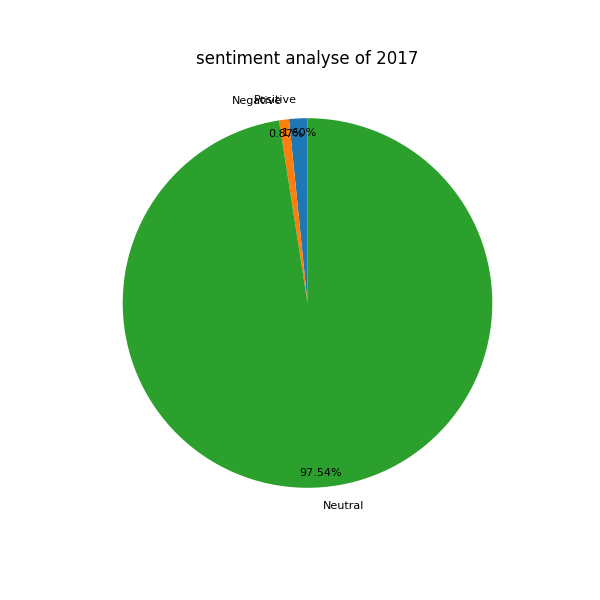
\includegraphics[width=0.75\textwidth]{../stats/Counts/sentimentchart2017.png}\\
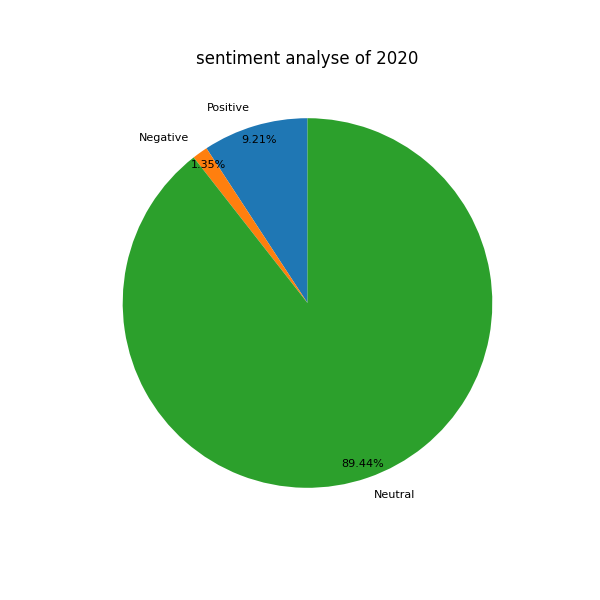
\includegraphics[width=0.75\textwidth]{../stats/Counts/sentimentchart2020.png}\\
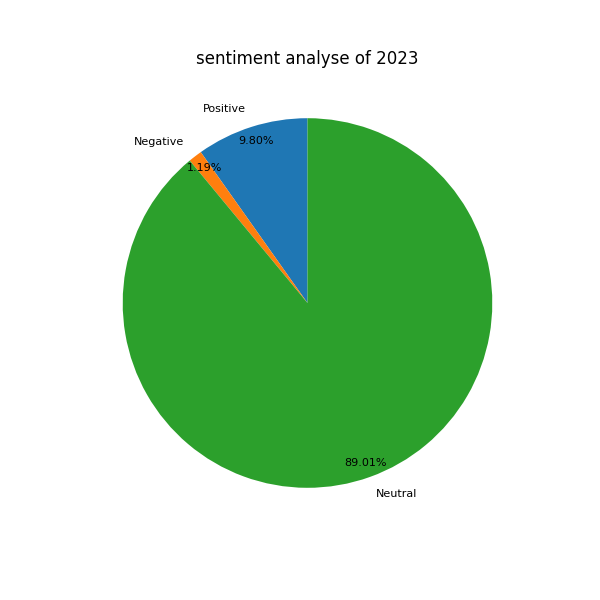
\includegraphics[width=0.75\textwidth]{../stats/Counts/sentimentchart2023.png}\\
\subsection{Top10 words of each label:}
\subsubsection{2017:}
\begin{align*}
	\csvautotabular{../stats/Top10/top10_2017.csv}
\end{align*} 
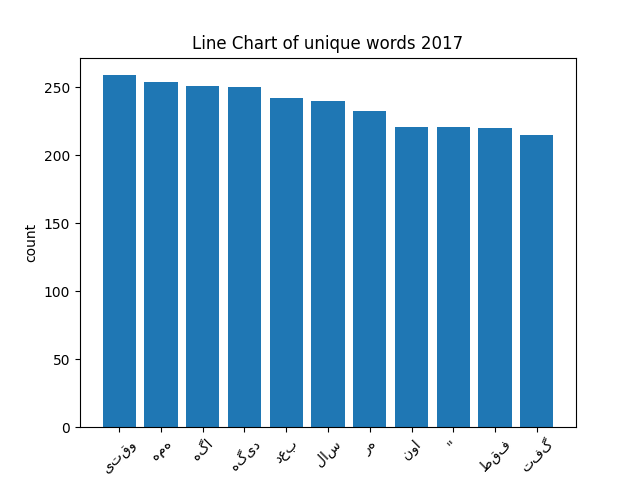
\includegraphics[width=0.75\textwidth]{../stats/Top10/top10chart2017.png}
\subsubsection{2020:}
\begin{align*}
	\csvautotabular{../stats/Top10/top10_2020.csv}
\end{align*} 
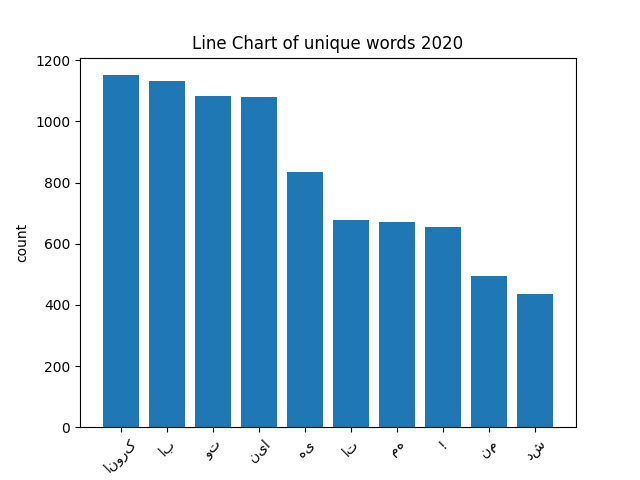
\includegraphics[width=0.75\textwidth]{../stats/Top10/top10chart2020.png}
\subsubsection{2023:}
\begin{align*}
	\csvautotabular{../stats/Top10/top10_2023.csv}
\end{align*} 
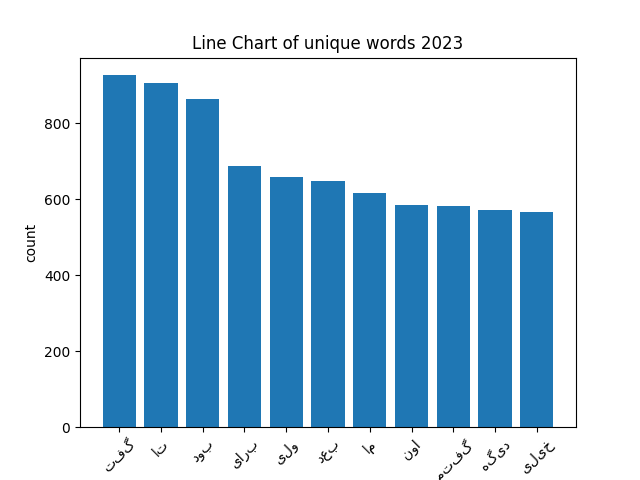
\includegraphics[width=0.75\textwidth]{../stats/Top10/top10chart2023.png}
\subsection{Common and Uncommon counts of words:}
\begin{align*}
	\csvautotabular{../stats/Common_Uncommon/common_count.csv}
\end{align*} 
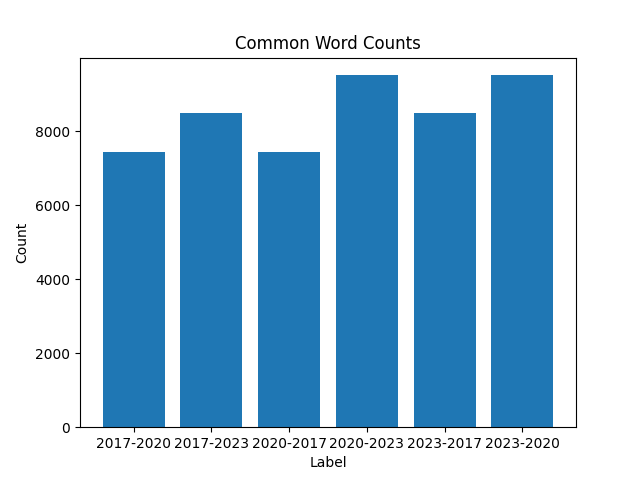
\includegraphics[width=1\textwidth]{../stats/Common_Uncommon/commonWords.png}\\
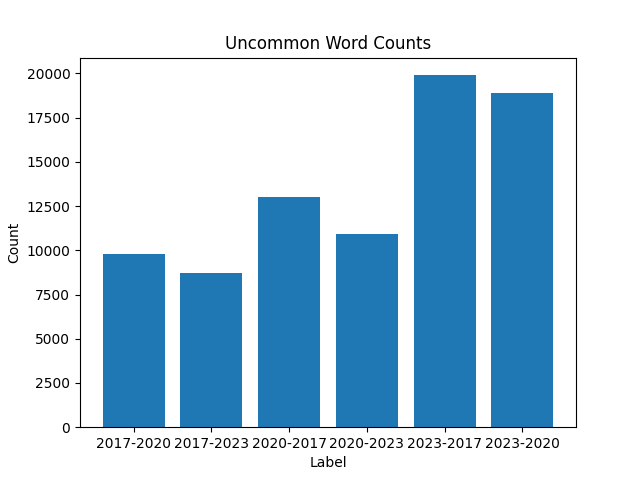
\includegraphics[width=1\textwidth]{../stats/Common_Uncommon/uncommonWords.png}\\
\bigskip

%------------------------------------------------
\subsection{Relative Normalized Frequency(RNF):}
\subsubsection{2017-2020 Common words by RNF}
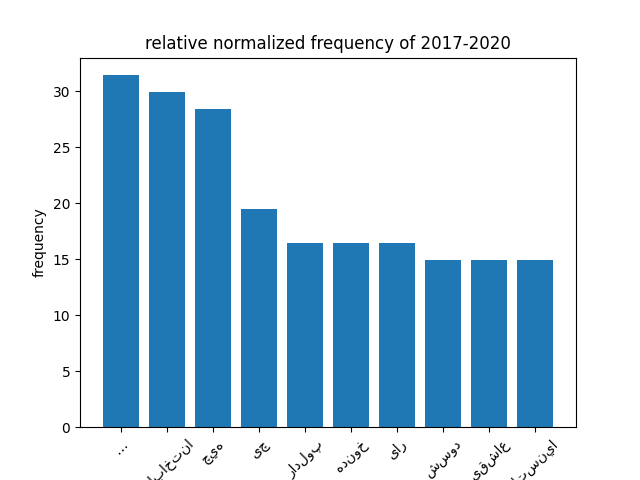
\includegraphics[width=0.8\textwidth]{../stats/RNF/rnf17_20.png}
\subsubsection{2017-2023 Common words by RNF}
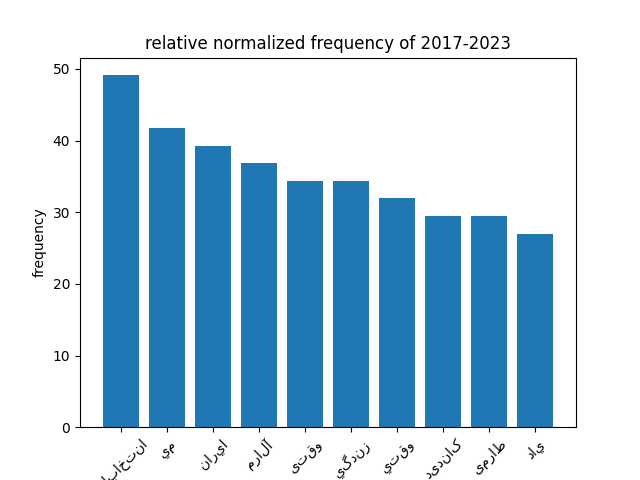
\includegraphics[width=0.8\textwidth]{../stats/RNF/rnf17_23.png}
\subsubsection{2020-2017 Common words by RNF}
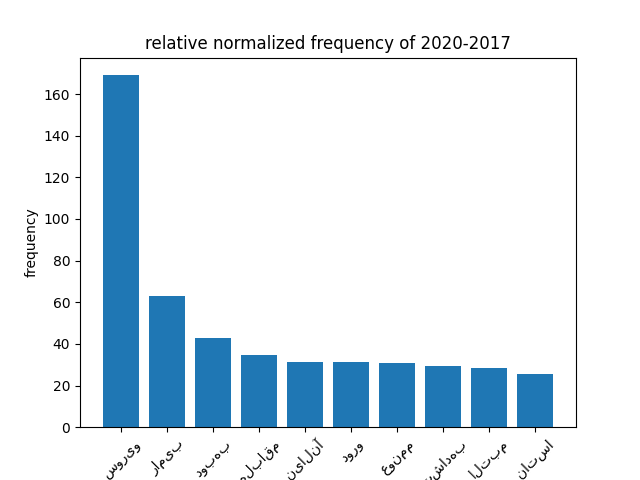
\includegraphics[width=0.8\textwidth]{../stats/RNF/rnf20_17.png}
\subsubsection{2020-2023 Common words by RNF}
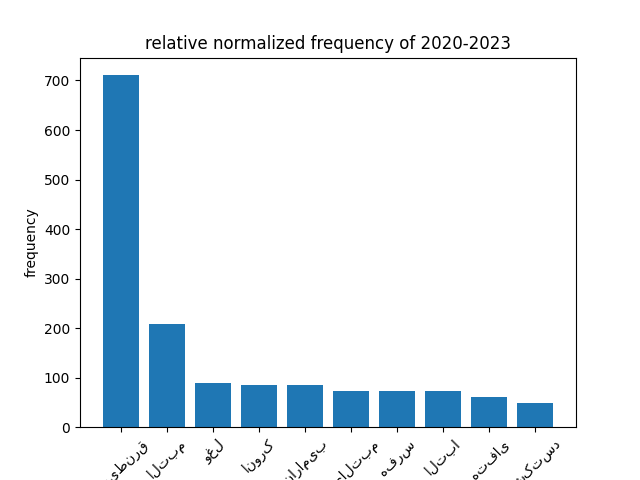
\includegraphics[width=0.8\textwidth]{../stats/RNF/rnf20_23.png}
\subsubsection{2023-2017 Common words by RNF}
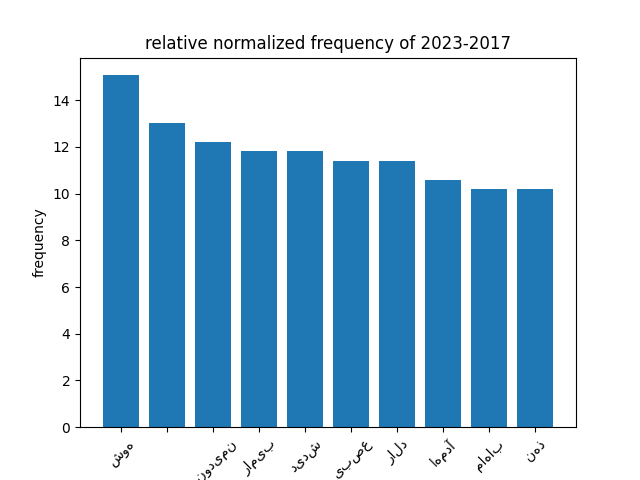
\includegraphics[width=0.8\textwidth]{../stats/RNF/rnf23_17.png}
\subsubsection{2023-2020 Common words by RNF}
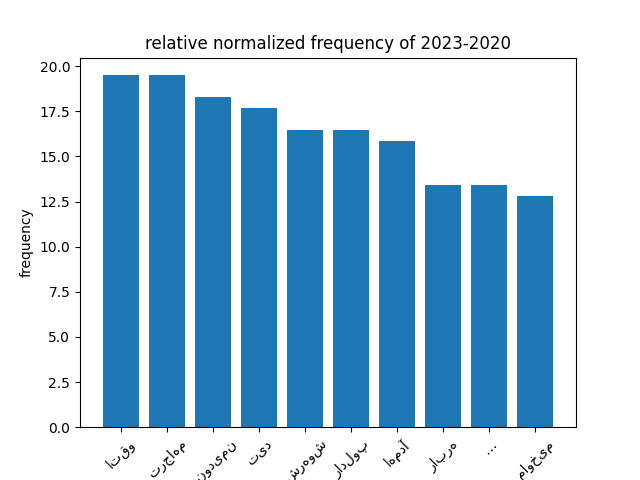
\includegraphics[width=0.8\textwidth]{../stats/RNF/rnf23_20.png}

%------------------------------------------------
\subsection{TF-IDF:}
\subsubsection{2017 tf-idf most Common words}
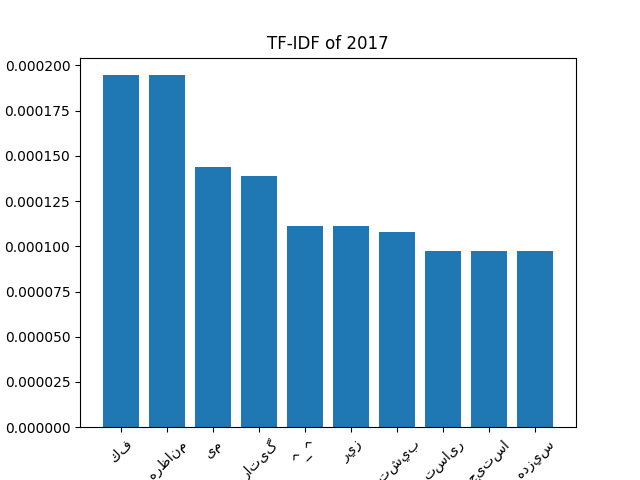
\includegraphics[width=0.8\textwidth]{../stats/TF-IDF/tfidf17.png}
\subsubsection{2020 tf-idf Common words}
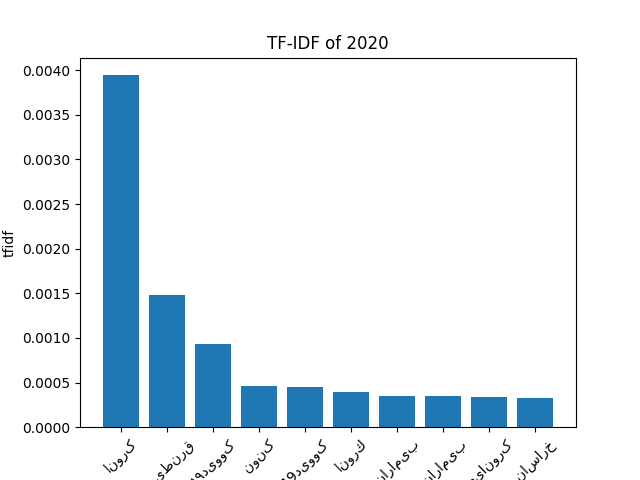
\includegraphics[width=0.8\textwidth]{../stats/TF-IDF/tfidf20.png}
\subsubsection{2023 tf-idf most Common words}
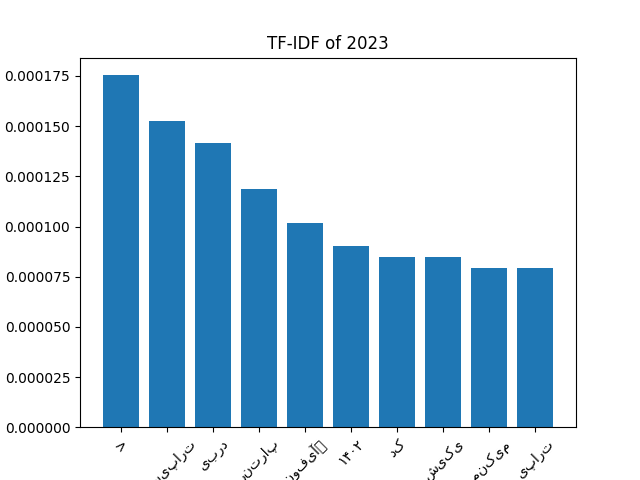
\includegraphics[width=0.8\textwidth]{../stats/TF-IDF/tfidf23.png}

\subsection{histogram of all word:}
\begin{align*}
	\csvautotabular{../stats/Histogram/top10_All.csv}
\end{align*} 
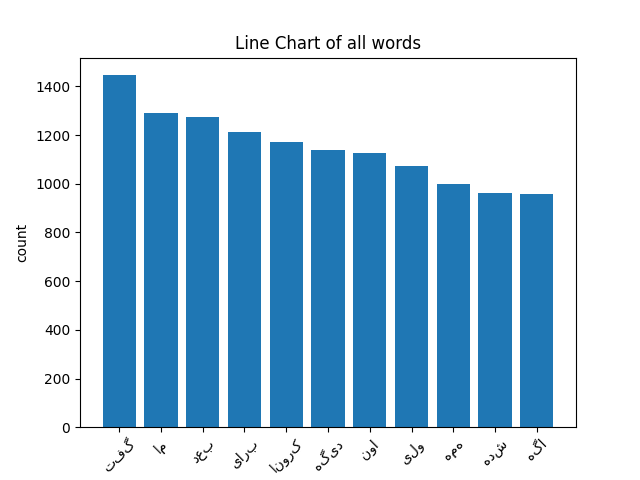
\includegraphics[width=1\textwidth]{../stats/Histogram/top10chartAll.png}

\pagebreak
\bibliography{ecl}
\bibliographystyle{apa6}
\end{document}